\documentclass[../hw.tex]{subfiles}
\begin{document}
\setcounter{section}{7}
\begin{center}
  \section*{Homework 7} \label{sec:homework7}
  \subsection*{Due 3/20}
\end{center}
\addcontentsline{toc}{section}{\nameref{sec:homework7}}
\hrule \vspace{10px}

\paragraph*{1.} (a) The center of mass is
\begin{align*}
    \vb R = \frac{m_1 \vb r_1 + m_2 \vb r_2}{m_1 + m_2} = \frac{1}{M} (m_1 \vb r_1 + m_2 \vb r_2) 
    \qquad M = m_1 + m_2
\end{align*}
we can rewrite the position vectors in terms of the COM and separation vector:
\begin{align*}
    \vb r_1 &= \vb R + \frac{m_2}{M} \vb r \\
    \vb r_2 &= \vb R - \frac{m_1}{M} \vb r
\end{align*}
Transforming into the CM frame since $\vb R$ is an ignorable coordinate ($\lagr$ doesn't depend on $\vb R$)
\begin{align*}
    \vb r_1' &= \vb r_1 - \vb R = \frac{m_2}{M} \vb r \\
    \vb r_2' &= \vb r_2 - \vb R = -\frac{m_1}{M} \vb r
\end{align*}
so The kinetic energy of the two particles are
\begin{align*}
    T_1 &= \frac{1}{2} m_1 \qt(\frac{m_2}{M} \dot{\vb r})^2 
    \qquad T_2 = \frac{1}{2} m_2 \qt(-\frac{m_1}{M} \dot{\vb r})^2 
\end{align*}
and the potential energy is
\begin{align*}
    U = \frac{1}{2} k r^2
\end{align*}
The Lagrangian in polar coordinates is
\begin{align*}
    \lagr &= T_1 + T_2 - U \\
    &= \frac{1}{2} \frac{m_1 m_2^2}{M^2} \dot{\vb r}^2 
        + \frac{1}{2} \frac{m_1^2 m_2}{M^2} \dot{\vb r}^2 - \frac{1}{2} k r^2  \\
    &= \frac{1}{2} \frac{m_1 m_2(m_1 + m_2)}{M(m_1 + m_2)} \dot{\vb r}^2 - \frac{1}{2} k r^2 \\
    &= \frac{1}{2} \mu \dot{\vb r}^2 - \frac{1}{2} k r^2 \qquad \mu = \frac{m_1 m_2}{m_1 + m_2} \\
    \lagr &= \frac{1}{2} \mu \qt(\dot{r}^2 + r^2 \dot{\phi}^2) - \frac{1}{2} k r^2
\end{align*}
(b) From the EL equation for we find a conserved quantity
\begin{align*}
    \pdv{\lagr}{\dot{\phi}} &= \mu r \dot \phi = \ell
\end{align*}
and
\begin{align*}
    \pdv{\lagr}{r} &= \mu r \dot\phi^2 - \pdv{U}{r} \\
    \dv{t}(\pdv{\lagr}{\dot r}) &= \mu \ddot{r} \\
    \implies \mu \ddot r &= \mu r \dot\phi^2 - \pdv{U}{r} \\
    &= \frac{\ell^2}{\mu r^3} - \pdv{U}{r} \qquad U = \frac{1}{2} k r^2
\end{align*}
rewriting the first term as the negative gradient of a potential i.e.
\begin{align*}
    \mu \ddot r &= -\pdv{r}(U_{cf} + U)
\end{align*}
\begin{align*}
    \frac{\ell^2}{\mu r^3} &= -\pdv{U_{cf}}{r} \\
    U_{cf} &= \frac{\ell^2}{2\mu r^2}
\end{align*}
so we have an effective potential
\begin{align*}
    U_{\text{eff}} &= U + U_{cf} \\
    &= \frac{1}{2} k r^2 + \frac{\ell^2}{2\mu r^2}
\end{align*}
\begin{figure}[ht]
    \centering
    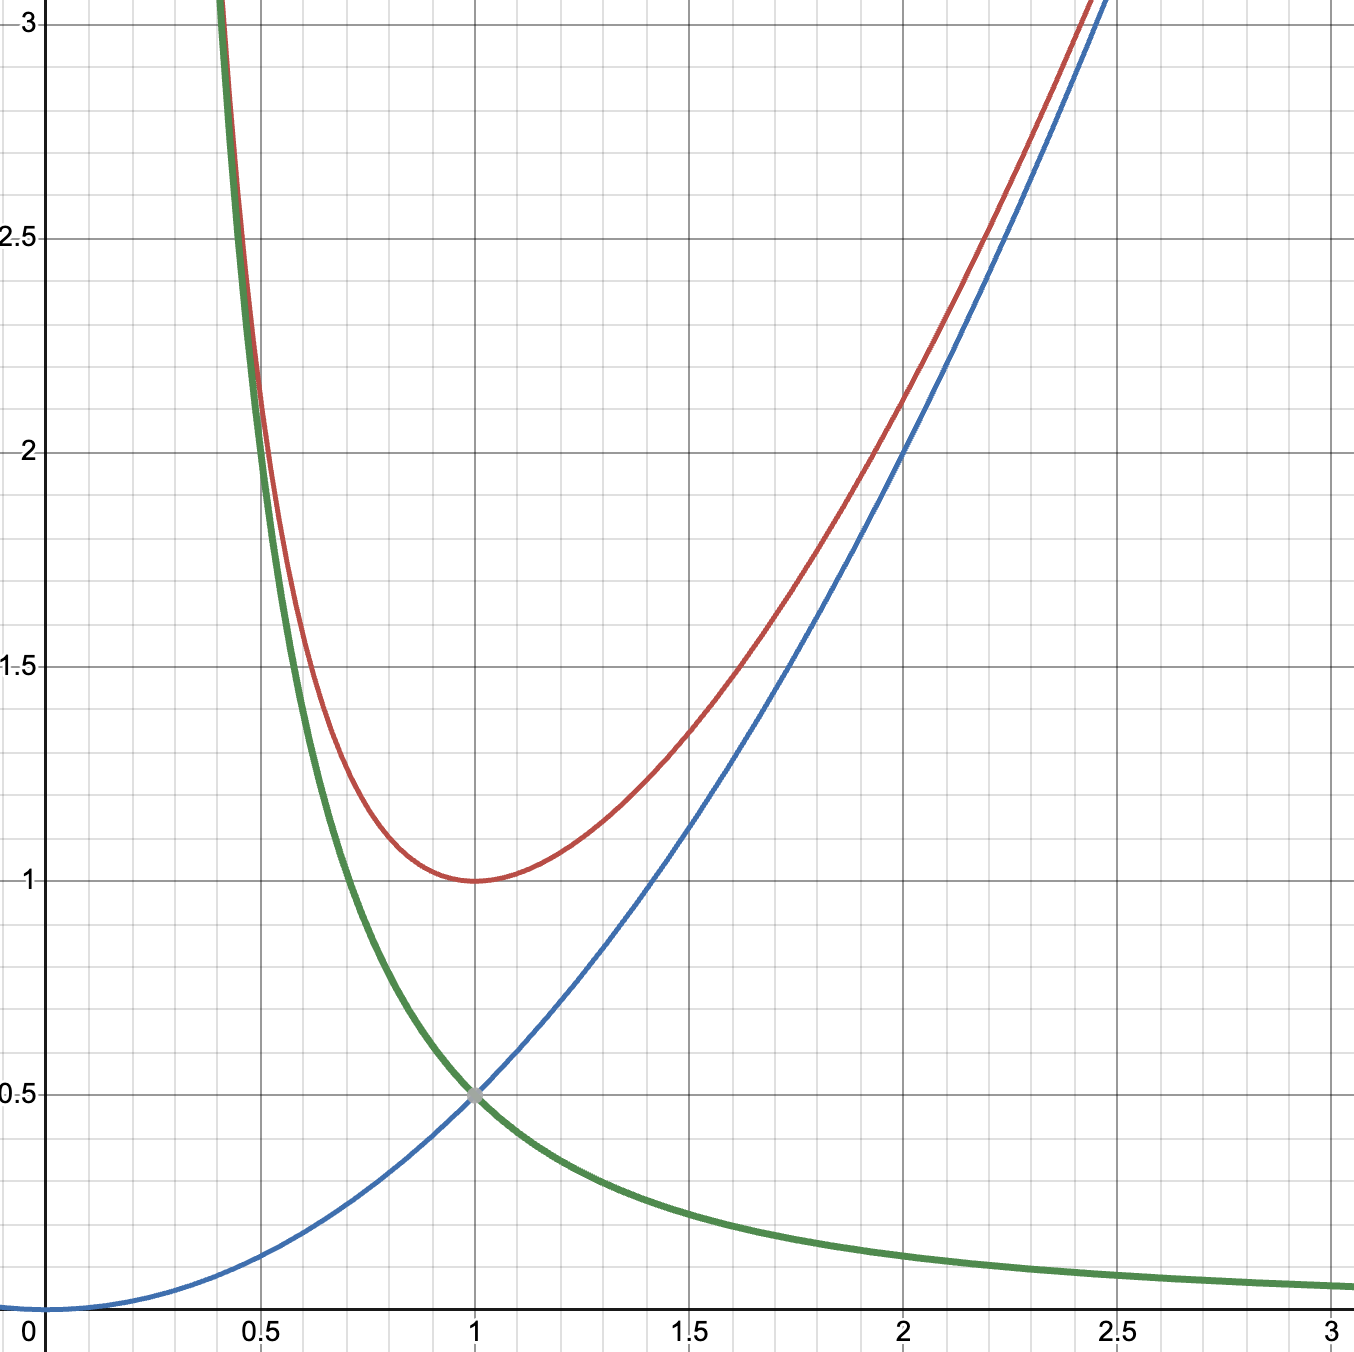
\includegraphics[width=0.5\textwidth]{hw7_potential.png}
    \caption{Effective potential $U_{\text{eff}}$ for the reduced mass in Red. $U_{cf}$ is in Green
    and $U$ is in Blue.}
    \label{fig:hw7_1}
\end{figure}

To find the equilibrium point, we find the minimum of $U_{\text{eff}}$ or when the derivative is zero:
\begin{align*}
    U'_{\text{eff}}(r_0) &= kr_0 - \frac{\ell^2}{\mu r_0^3} = 0 \\
    kr_0 &= \frac{\ell^2}{\mu r_0^3} \\
    r_0^4 &= \frac{\ell^2}{\mu k} \\
    r_0 &= \qt(\frac{\ell^2}{\mu k})^{1/4}
\end{align*}
We can see from the sketch that $r_0$ is a stable equilibrium point.

(c) Taylor expanding the effective potential about $r_0$:
\begin{align*}
    U_{\text{eff}}(r) &\approx U_{\text{eff}}(r_0) + (r - r_0)U'_{\text{eff}}(r_0) + \frac{1}{2}(r - r_0)^2 U''_{\text{eff}}(r_0) \\
\end{align*}
When we set the reference point at $r_0$, the first term is zero, the second term is zero from
part (b), so the third term is
\begin{align*}
    U''_{\text{eff}}(r_0) &= k + \frac{3\ell^2}{\mu r_0^4} \\
    &= k + \frac{3\ell^2}{\mu}\frac{1}{\qt(\frac{\ell^2}{\mu k})} \\
    &= k + 3k \\
    &= 4k \\
    \implies U_{\text{eff}}(r) &\approx \frac{1}{2} (4k) \Delta r^2 \qquad \Delta r = r - r_0
\end{align*}
which would give the equation of motion 
\begin{align*}
    \mu \ddot{\Delta r} &= -4k \Delta r
\end{align*}
with a frequency of
\begin{align*}
    \omega &= \sqrt{\frac{4k}{\mu}}
\end{align*}
The periodicity of the motion implies closed orbit?

\newpage
\paragraph*{2.} (a) Given $U = kr^n$, the negative gradient of the potential is the force:
\begin{align*}
    F = -\grad U = - \pdv{U}{r} = - kn r^{n-1} = - \frac{n}{r} U
\end{align*}
where the magnitude of force is also equivalent to the centripetal force $F = -mv^2/r$ (the sign
specifies the inward direction). Therefore,
\begin{align*}
    -\frac{mv^2}{r} &= -\frac{n}{r} U \\
    mv^2 &= n U
\end{align*}
Subbing into the KE equation
\begin{align*}
    T = \frac{1}{2} mv^2 = \frac{1}{2} nU
\end{align*}
(b) Given $G = \vb r \cdot \vb p$, taking the time derivative of $G$:
\begin{align}
    \dv{t} G &= \dot{\vb r} \cdot \vb p + \vb r \cdot \dot{\vb p} \\
    &= mv^2 + \vb F \cdot \vb r \\
    &= 2T + \vb F \cdot \vb r
\end{align}
and integrating from $t = 0 \to t$ ():
\begin{align*}
    \int_0^t 2 T + \vb F \cdot \vb r \dd{t} &= \int_0^t \dv{t} G \dd{t} \\
    &= G(t) - G(0)
\end{align*}
and diving by $t$:
\begin{align*}
    \frac{G(t) - G(0)}{t} &= 2 \frac{1}{t} \int_0^t T \dd{t} + \frac{1}{t} \int_0^t \vb F \cdot \vb r \dd{t} \\
    &= 2 \expval{T} + \expval{\vb F \cdot \vb r}
\end{align*}
(c) Letting $U = kr^n$, we can find the force:
\begin{align*}
    \vb F &= -\grad U = -\pdv{U}{r} = -kn r^{n-1} \vu r = -\frac{n}{r} U \vu r
\end{align*}
so the work done is
\begin{align*}
    \vb F \cdot \vb r = -n U
\end{align*}
So in the equation from (b) for $t \to \infty$
\begin{align*}
    \frac{G(t) - G(0)}{t} = 0
\end{align*}
the left side goes to zero and
\begin{align*}
    0 &= 2 \expval{T} + \expval{-nU}
\end{align*}
and since $n$ is some constant
\begin{align*}
    0 &= 2 \expval{T} - n \expval{U} \\
    \implies \expval{T} &= \frac{n}{2} \expval{U}
\end{align*}

\newpage
\paragraph*{3.} (a) 
\end{document}